%; whizzy document
% latex beamer presentation.
% platex, latex-beamer でコンパイルすることを想定。 


%     Tokyo Debian Meeting resources
%     Copyright (C) 2006 Junichi Uekawa

%     This program is free software; you can redistribute it and/or modify
%     it under the terms of the GNU General Public License as published by
%     the Free Software Foundation; either version 2 of the License, or
%     (at your option) any later version.

%     This program is distributed in the hope that it will be useful,
%     but WITHOUT ANY WARRANTY; without even the implied warranty of
%     MERCHANTABILITY or FITNESS FOR A PARTICULAR PURPOSE.  See the
%     GNU General Public License for more details.

%     You should have received a copy of the GNU General Public License
%     along with this program; if not, write to the Free Software
%     Foundation, Inc., 51 Franklin St, Fifth Floor, Boston, MA  02110-1301 USA

% 実行順番
% sudo  ~/bin/usb-macbook-ir.c &
% real presentation (shell-command (concat "DISPLAY=:0.1 xpdf -fullscreen " (replace-regexp-in-string "tex$" "pdf"(buffer-file-name)) "&"))
% DISPLAY=:0.1 xpdf -fullscreen 

\documentclass[cjk,dvipdfmx]{beamer}
\usetheme{Warsaw}
%  preview (shell-command (concat "xpdf " (replace-regexp-in-string "tex$" "pdf"(buffer-file-name)) "&"))
%  presentation (shell-command (concat "xpdf -fullscreen " (replace-regexp-in-string "tex$" "pdf"(buffer-file-name)) "&"))

%http://www.naney.org/diki/dk/hyperref.html
%日本語EUC系環境の時
\AtBeginDvi{\special{pdf:tounicode EUC-UCS2}}
%シフトJIS系環境の時
%\AtBeginDvi{\special{pdf:tounicode 90ms-RKSJ-UCS2}}

\title{Mactel Debian の深遠なる世界}
%\title[Debian 勉強会クイズ問題]{Debian勉強会クイズ}
\subtitle{OSC 2006 Hokkaido}
\author{東京エリア Debian勉強会\\ 上川 純一 dancer@debian.org\\IRC nick: dancerj}
\date{2006年7月15日}

% 三択問題用
\newcounter{santakucounter}
\newcommand{\santaku}[5]{%
\addtocounter{santakucounter}{1}
\frame{\frametitle{問題\arabic{santakucounter}. #1}
%問題\arabic{santakucounter}. #1
\begin{minipage}[t]{0.7\hsize}
 \begin{itemize}
 \item □ A #2\\
 \item □ B #3\\
 \item □ C #4\\
 \end{itemize}
\end{minipage}
}
\frame{\frametitle{問題\arabic{santakucounter}. #1}
%問題\arabic{santakucounter}. #1
\begin{minipage}[t]{0.7\hsize}
\begin{itemize}
\item □ A #2\\
\item □ B #3\\
\item □ C #4\\
\end{itemize}
\end{minipage}
\begin{minipage}[t]{0.2\hsize}
答えは:


\vspace{1cm}

{\huge \hspace{1cm}#5}
\end{minipage}}
}


\begin{document}
\frame{\titlepage{}}



\section{Debian 勉強会}

\begin{frame}
\frametitle{ここにいる人達は誰?}
\begin{itemize}[<+->]
 \item 岩松さん
 \item superHハッカー\\
       Debian Developerになるべく修行中
 \item 上川 純一
 \item Debian Developer
\end{itemize}
\end{frame}

\begin{frame}
 \frametitle{Debian Project}
 \begin{itemize}[<+->]
  \item Debian Projectとは何?
  \item Linux distributionを作成するプロジェクト、1993年ころ発足
  \item 1日1回 unstable リリースがリリースされる
  \item 10以上のCPUアーキテクチャをサポート
  \item 30人程度の日本人開発者
  \item 1000人の開発者、世界中に分散
  \item 20000くらいのパッケージ数
 \end{itemize}
\end{frame}

\begin{frame}
\frametitle{Debian勉強会}
\begin{itemize}
 \item 2005年1月開始
 \item Debian Developer 上川発起人
 \item 東京の公民館で月に一回コンスタントに開催
\end{itemize}
\end{frame}



\begin{frame}
\frametitle{Debian勉強会:解決したい内容}
\begin{itemize}
 \item<1-> 問題
       \begin{itemize}
	\item 現状MLとIRCで情報交換している
	\item face-to-faceであう場所がない
	\item まとまったドキュメントが出てこない
       \end{itemize}
 \item<2-> Debian勉強会の提案
       \begin{itemize}
	\item 定期的に集まる
	\item 資料を必ず作成する。(GPLで!)
       \end{itemize}
\end{itemize}
\end{frame}

\begin{frame}
 \frametitle{Debian勉強会:実際}
 \begin{itemize}
  \item Debian Weekly News Quiz
  \item パッケージング関連の話題など専門の人に話をきく
  \item 前回の内容:\\
	debian conference 2006 の参加報告\\
	参加してハックした結果(cowdancer)の報告
  \item 今回の目的:Debian 勉強会の雰囲気をあじわってください。
 \end{itemize}
\end{frame}


\santaku
{mozilla はどうなるか}
{サポートされなくなるので削除され、xulrunnerに移行が必要}
{mozillaは永遠です}
{使いにくいのでIEに置き換える}
{A}

\santaku
{Debconf6 は何回目のDebconfか。}
{4}
{6}
{7}
{C}


\section{Debian on Macbookの意義}

\begin{frame}
\frametitle{Debian on MacBook 新規性}
\begin{center}
\begin{minipage}{0.5\hsize}
  \begin{itemize}
   \item 新アーキテクチャ\\
	起動部分がEFI管理\\
	変なアーキテクチャのマシンをいじりたい!

   \item 内蔵キーボード、iSight、リモコン、あらゆるものがUSB接続
   \item Intel Core Duo: dual-core CPU
 \end{itemize}
\end{minipage}
\end{center}
\end{frame}

\begin{frame}
\frametitle{EFIという福音}

\begin{tabular}[t]{|p{8em}|p{8em}|p{8em}|}
\hline
 & BIOS & EFI \\
\hline
パーティション & MBR:4個 (「基本」) & GPT: 128 \\
\hline
ファイルシステム & 魔窟 & FAT を読める \\
\hline
実行フォーマット & なにそれ? & PE32+形式の実行ファイル\\
\hline
\end{tabular}
\end{frame}


\begin{frame}
\frametitle{EFIコマンドライン}

MS DOS 風味のコマンドラインが利用できるようになる。\\
ブートローダ以前の段階でコマンドラインが利用できるように!

EFI$>$ fs0:\\
EFI fs0:$>$ cd EFI\\
EFI fs0:$\backslash{}$EFI$>$ cd dancer\\
EFI fs0:$\backslash{}$EFI$\backslash{}$dancer$>$ cd refit\\
EFI fs0:$\backslash{}$EFI$\backslash{}$dancer$\backslash{}$refit$>$ dir\\
refit.efi\\
 EFI fs0:$\backslash{}$EFI$\backslash{}$debian$\backslash{}$refit$>$ refit

\end{frame}

\section{Debian on Macbook}

\begin{frame}
 \frametitle{MacBookへのMac OS X と Debian の dual-boot 設定}
 \begin{minipage}{0.5\hsize}
  \begin{itemize}
   \item MacBook 購入
   \item Mac OS X からのパーティション処理
   \item rEFIt のインストール
   \item Debian のインストール
   \item 各種設定
  \end{itemize}
 \end{minipage}
\end{frame}

\subsection{MacBook 購入} 

\begin{frame}
 \frametitle{MacBook 購入}
 \begin{minipage}{0.5\hsize}
  \begin{itemize}
   \item クリックするだけ!
  \end{itemize}
 \end{minipage}
\end{frame}

\subsection{Mac OS X からのパーティション処理}

\begin{frame}
 \frametitle{Mac OS X からのパーティション処理}
\begin{itemize}
 \item 最近の Mac OS X ではファイルシステムのオンラインリサイズ可能\\
       \texttt{Mac OS X$\sharp$  sudo diskutil resizevolume disk0s2 20G}
\end{itemize}
\end{frame}

\subsection{rEFIt のインストール}

\begin{frame}
 \frametitle{rEFIt のインストール}
 \begin{itemize}
  \item MacOS X 上で bless 実行、起動時にrEFItが実行されるようにする
  \item \url{http://refit.sourceforge.net/}からバイナリをダウンロードし
	た場合
  \begin{itemize}
   \item \texttt{/efi}など、適当な場所ににファイルを展開
   \item \texttt{./enable.sh}を実行 (\texttt{bless}を実行するスクリプト)
  \end{itemize} 
  \item Debian パッケージ refit の中身を利用する場合
  \begin{itemize}
   \item refitパッケージの\texttt{/usr/lib/refit/}以下をMac OS X 上にコピー
   \item \texttt{sudo bless --folder [refit.efiのあるディレクトリへのフルパス] --file [refit.efiへのフルパス]}
  \end{itemize}
 \item 再起動するとrEFItの画面が出るように
 \end{itemize}
\end{frame}

\begin{frame}
\frametitle{起動シーケンス}
\begin{minipage}[t]{0.4\hsize}
% dot -Tps -o bootchain.ps bootchain.dot
\includegraphics[height=1\hsize]{image200607/bootchain.ps}
\end{minipage}
\begin{minipage}[t]{0.58\hsize}
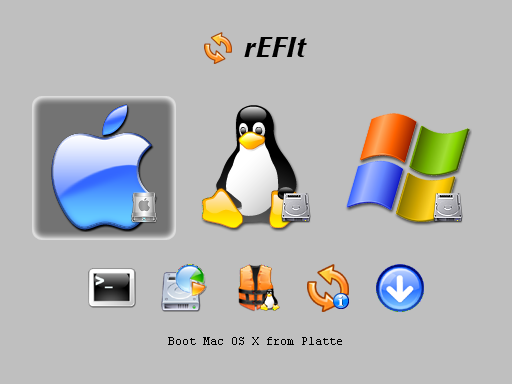
\includegraphics[width=1\hsize]{image200607/screen1.png}
\end{minipage}
\end{frame}

\subsection{Debian のインストール}

\begin{frame}
 \frametitle{Debian のインストール}
\begin{itemize}
 \item 2006年7月版以降のetchならどうやら動くでしょう\\
       インストール先はパーティション番号3か4にするのに注意
 \item ブートローダはliloを指定するのだが、現状そのままでは動かない
 \item parted が動作してパーティションを切ったあと、GPTパーティションを
       作成し、MBRが破壊されている\\
       Alt-F2でコマンドコンソールへ移動\\
       gptsync コマンドを利用して同期させ\\
       Alt-F1でもどる
 \item lilo をパーティションにインストール
 \item リブートするとrEFItからLinuxが起動可能に
\end{itemize}
\end{frame}

\begin{frame}
\frametitle{MBR と GPT での見えかた例}
同じディスクであっても見えかたが違う\\
\begin{minipage}[t]{0.68\hsize} 
MBR

{\scriptsize
 Disk /dev/sda: 80.0 GB, 80026361856 bytes\\
255 heads, 63 sectors/track, 9729 cylinders\\
Units = cylinders of 16065 * 512 = 8225280 bytes\\

   Device Boot      Start         End      Blocks   Id  System\\
/dev/sda1               1          26      204819+  ee  EFI GPT\\
/dev/sda2              26        2637    20971520   af  Unknown\\
/dev/sda3   *        2637        2758      976563   ef  EFI (FAT-12/16/32)\\
/dev/sda4            2758        5190    19531250+  ef  EFI (FAT-12/16/32)\\
}
\end{minipage}
\begin{minipage}[t]{0.30\hsize}
GPT\\

{\small
 major minor  $\sharp{}$blocks  name\\

   8     0   78150744 sda\\
   8     1     204800 sda1\\
   8     2   20971520 sda2\\
   8     3     976563 sda3\\
   8     4   19531250 sda4\\
   8     5    2929688 sda5\\
}
\end{minipage}
\end{frame}

\subsection{各種設定}

\begin{frame}
 \frametitle{Xの設定}
\begin{itemize}
 \item i810ドライバで簡単設定
 \item 915resolution で 1280x800に設定
 \item マウスの右ボタンなどがないので、xkbsetで対応
\end{itemize}
\end{frame}

\begin{frame}
 \frametitle{カーネルの設定}
\begin{itemize}
 \item 2.6.17以前のカーネルは5回に1回程度パニックするので注意
 \item 2.6.17時点で、rtc.ko は対応していないようなので、rtc-dev.ko など
       を利用
 \item サウンドカード:\texttt{snd\_hda\_intel}
 \item ネットワークカード: 有線は、sky2\\
       無線は madwifi
 \item CPUは \texttt{speedstep\_centrino} で周波数制御可能、
       \texttt{apt-get install cpufreqd}
\end{itemize}
\end{frame}

\begin{frame}
 \frametitle{madwifi}
 \begin{itemize}
  \item \texttt{sudo apt-get install madwifi-source madwifi-tools madwifi-doc}
  \item \texttt{sudo m-a prepare}
  \item \texttt{sudo m-a a-i madwifi}
  \item \texttt{sudo modprobe ath\_pci}
  \item<2-> たまに起動時にハングします
 \end{itemize}
\end{frame}

\begin{frame}
 \frametitle{linux-uvc}
 \begin{itemize}
  \item \texttt{sudo apt-get install linux-uvc-source linux-uvc-tools}
  \item \texttt{sudo m-a prepare}
  \item \texttt{sudo m-a a-i linux-uvc}
  \item \texttt{sudo macbook-isight-firmware-loader \\
       /mnt/mac/System/Library/Extensions/IOUSBFamily.kext/Contents/PlugIns\\/AppleUSBVideoSupport.kext/Contents/MacOS/AppleUSBVideoSupport}
  \item \texttt{sudo modprobe uvcvideo}
  \item \texttt{sudo apt-get install ekiga libpt-plugins-v4l2}
 \end{itemize}
\end{frame}

\section{副次的な目標}

\subsection{どんなハックをしたか}

\begin{frame}
 \frametitle{この発表のために仕込んだパッチ}

 発表をするためにDebianを使い込む

 \begin{itemize}[<+->]
  \item 377198: module-assistant: カーネルモジュールがカーネル2.6.18-rc1ではコンパイルでき
	ない
  \item 247602: xpdf-reader: metacityでのフルスクリーンになるようにする
	パッチ
  \item IR receiver hack: プレゼンテーションをリモコンで実施するため
  \item Debian refit パッケージ作成
  \item linux-uvc パッケージ作成
 \end{itemize}
\end{frame}

\subsection{たとえばリモコン}

\begin{frame}
 \frametitle{USBデバイス}

\begin{minipage}[t]{0.4\hsize}
  \begin{itemize}
  \item<1-> リモコン付属
  \item<1-> USB HID デバイス
  \item<2-> libusbとlibXtst\\
       3分ハッキング
  \item<3-> カーネルドライバがすでに存在しているので実はxmodmapだけで実装で
	きる
 \end{itemize}
\end{minipage}
\begin{minipage}[t]{0.5\hsize}
 \onslide<2->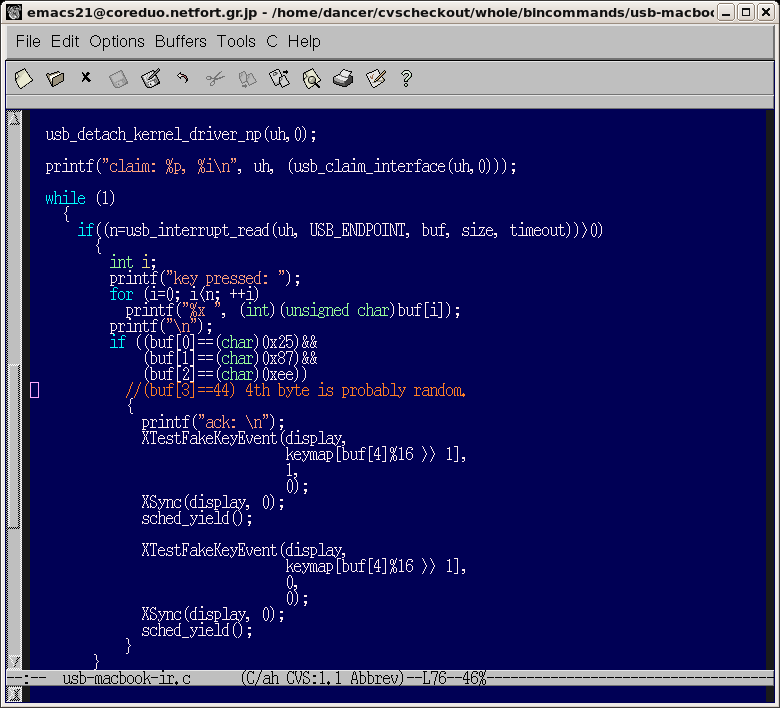
\includegraphics[width=2\hsize]{image200607/usbir.png}
\end{minipage}
\end{frame}



\begin{frame}
\frametitle{最後に}
まだうまくうごいていないデバイス一覧
\begin{itemize}
 \item suspend/sleep
 \item CD-Rの動作にはパッチが必要という噂
 \item バックライトについては最近ドライバが出てきましたが、MacBookで動く
       のか?
 \item bluetooth については未検証
 \item その他、気づいていない機能
\end{itemize}
\end{frame}

%
%
%
%

\begin{frame}
\frametitle{おまけスライド}
\end{frame}

\begin{frame}
\frametitle{できたこと}
\begin{itemize}
 \item rEFItをDebian上でコンパイルできるように
 \item refit Debianパッケージの作成、アップロード (375999)
 \item それっぽく動作試験
 \item gptsyncコマンドの提供
\end{itemize}
\end{frame}

\begin{frame}
\frametitle{できてないこと}
\begin{itemize}
 \item インストール手法の確立\\
       MacOSXのbless コマンドに依存しない方法がない
 \item debian-installerへの統合
 \item rEFItでコンパイルできないツール多数\\
       gptsync.efiが動作していない -- 7/8 修正済み\\
       gnu-efiのefilibがどうも古いようだ(376000)
 \item バイナリ配布されているツールの発見(ソースはどこ?)
 \item elilo がうまくうごかない (376002)
 \item Debianの2.6.16/2.6.17カーネルは
       よくカーネルパニックをおこす\\
       (Linusの7月2日,8日のgitツリーは安定動作、Mactel用のパッチが多数マージ
       されているようなのでお薦め)
\end{itemize}
\end{frame}

\begin{frame}
\frametitle{MBR vs GPT}
\begin{minipage}[t]{0.65\hsize} 
{\scriptsize
 Disk /dev/sda: 80.0 GB, 80026361856 bytes\\
255 heads, 63 sectors/track, 9729 cylinders\\
Units = cylinders of 16065 * 512 = 8225280 bytes\\

   Device Boot      Start         End      Blocks   Id  System\\
/dev/sda1               1          26      204819+  ee  EFI GPT\\
/dev/sda2              26        2637    20971520   af  Unknown\\
/dev/sda3   *        2637        2758      976563   ef  EFI (FAT-12/16/32)\\
/dev/sda4            2758        5190    19531250+  ef  EFI (FAT-12/16/32)\\
}
\end{minipage}
\begin{minipage}[t]{0.30\hsize}
{\small
 major minor  $\sharp{}$blocks  name\\

   8     0   78150744 sda\\
   8     1     204800 sda1\\
   8     2   20971520 sda2\\
   8     3     976563 sda3\\
   8     4   19531250 sda4\\
   8     5    2929688 sda5\\
}
\end{minipage}
\end{frame}

\begin{frame}
 \frametitle{EFI上でのgptsync実行例}
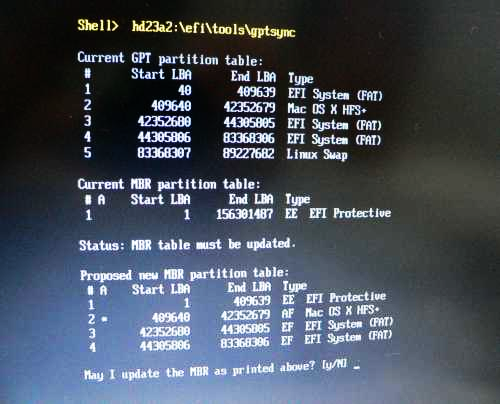
\includegraphics[width=0.8\hsize]{image200607/gptsync.png}
\end{frame}

\begin{frame}
 \frametitle{}
\begin{itemize}
 \item hfsplus -- HFS plus ファイルシステム
 \item hfsplus カーネルモジュール -- HFS plus ファイルシステム
 \item hfsutils -- HFS 
 \item \url{http://ipodlinux.org/Installation_from_Linux_Hfsplus}
 \item \url{http://darwinsource.opendarwin.org/tarballs/apsl/bless-37.tar.gz}
\end{itemize}
\end{frame}

\end{document}
